\section{Date: 2026-08-20}
\noindent \textbf{Series ID: CANRECM} 

\noindent This series is titled OECD based Recession Indicators for Canada from the Peak through the Trough (DISCONTINUED) and has a frequency of Monthly. The units are +1 or 0 and the seasonal adjustment is Not Seasonally Adjusted.The observation start date is 1960-02-01 and the observation end date is 2022-09-01.The popularity of this series is 9. \\ 

\noindent \textbf{Series ID: SFTPAGRM158SFRBSF} 

\noindent This series is titled San Francisco Tech Pulse (DISCONTINUED) and has a frequency of Monthly. The units are Percent Change at Annual Rate and the seasonal adjustment is Seasonally Adjusted.The observation start date is 1971-05-01 and the observation end date is 2020-03-01.The popularity of this series is 6. \\ 

\subsection{Raw Regression}
\noindent Regresses the two series against each other directly. A significant result here can come just as easily from both series sharing a long-run trend as from any real relationship.

\begin{center}
\begin{tabular}{lclc}
\toprule
\textbf{Dep. Variable:}       & value\_fred\_SFTPAGRM158SFRBSF & \textbf{  R-squared:         } &     0.070   \\
\textbf{Model:}               &              OLS               & \textbf{  Adj. R-squared:    } &     0.068   \\
\textbf{Method:}              &         Least Squares          & \textbf{  F-statistic:       } &     43.81   \\
\textbf{Date:}                &        Thu, 20 Aug 2026        & \textbf{  Prob (F-statistic):} &  8.18e-11   \\
\textbf{Time:}                &            12:21:40            & \textbf{  Log-Likelihood:    } &    184.44   \\
\textbf{No. Observations:}    &                587             & \textbf{  AIC:               } &    -364.9   \\
\textbf{Df Residuals:}        &                585             & \textbf{  BIC:               } &    -356.1   \\
\textbf{Df Model:}            &                  1             & \textbf{                     } &             \\
\textbf{Covariance Type:}     &           nonrobust            & \textbf{                     } &             \\
\bottomrule
\end{tabular}
\begin{tabular}{lcccccc}
                              & \textbf{coef} & \textbf{std err} & \textbf{t} & \textbf{P$> |$t$|$} & \textbf{[0.025} & \textbf{0.975]}  \\
\midrule
\textbf{const}                &       0.1539  &        0.009     &    16.656  &         0.000        &        0.136    &        0.172     \\
\textbf{value\_fred\_CANRECM} &      -0.0999  &        0.015     &    -6.619  &         0.000        &       -0.130    &       -0.070     \\
\bottomrule
\end{tabular}
\begin{tabular}{lclc}
\textbf{Omnibus:}       &  7.955 & \textbf{  Durbin-Watson:     } &    0.099  \\
\textbf{Prob(Omnibus):} &  0.019 & \textbf{  Jarque-Bera (JB):  } &    9.420  \\
\textbf{Skew:}          &  0.172 & \textbf{  Prob(JB):          } &  0.00901  \\
\textbf{Kurtosis:}      &  3.517 & \textbf{  Cond. No.          } &     2.43  \\
\bottomrule
\end{tabular}
%\caption{OLS Regression Results}
\end{center}

Notes: \newline
 [1] Standard Errors assume that the covariance matrix of the errors is correctly specified.

\begin{figure}
\centering
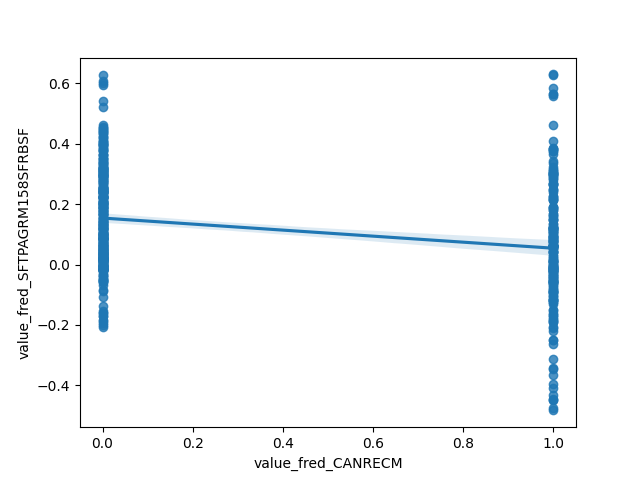
\includegraphics[scale = 0.9]{plots/plot_2026-08-20.png}
\caption{Raw Regression Plot for 2026-08-20}
\end{figure}
\newpage
\subsection{Detrended Regression}
\noindent Regresses the residuals of each series after removing its own linear time trend, so a shared trend can no longer drive the result on its own. A relationship that stays significant here is better evidence of a genuine link between the two series.

\begin{center}
\begin{tabular}{lclc}
\toprule
\textbf{Dep. Variable:}                  & value\_fred\_SFTPAGRM158SFRBSF\_detrended & \textbf{  R-squared:         } &     0.074   \\
\textbf{Model:}                          &                    OLS                    & \textbf{  Adj. R-squared:    } &     0.073   \\
\textbf{Method:}                         &               Least Squares               & \textbf{  F-statistic:       } &     46.95   \\
\textbf{Date:}                           &              Thu, 20 Aug 2026             & \textbf{  Prob (F-statistic):} &  1.85e-11   \\
\textbf{Time:}                           &                  12:21:40                 & \textbf{  Log-Likelihood:    } &    255.99   \\
\textbf{No. Observations:}               &                      587                  & \textbf{  AIC:               } &    -508.0   \\
\textbf{Df Residuals:}                   &                      585                  & \textbf{  BIC:               } &    -499.2   \\
\textbf{Df Model:}                       &                        1                  & \textbf{                     } &             \\
\textbf{Covariance Type:}                &                 nonrobust                 & \textbf{                     } &             \\
\bottomrule
\end{tabular}
\begin{tabular}{lcccccc}
                                         & \textbf{coef} & \textbf{std err} & \textbf{t} & \textbf{P$> |$t$|$} & \textbf{[0.025} & \textbf{0.975]}  \\
\midrule
\textbf{const}                           &   -1.755e-15  &        0.006     & -2.71e-13  &         1.000        &       -0.013    &        0.013     \\
\textbf{value\_fred\_CANRECM\_detrended} &      -0.0917  &        0.013     &    -6.852  &         0.000        &       -0.118    &       -0.065     \\
\bottomrule
\end{tabular}
\begin{tabular}{lclc}
\textbf{Omnibus:}       & 16.059 & \textbf{  Durbin-Watson:     } &    0.124  \\
\textbf{Prob(Omnibus):} &  0.000 & \textbf{  Jarque-Bera (JB):  } &   17.972  \\
\textbf{Skew:}          & -0.338 & \textbf{  Prob(JB):          } & 0.000125  \\
\textbf{Kurtosis:}      &  3.528 & \textbf{  Cond. No.          } &     2.07  \\
\bottomrule
\end{tabular}
%\caption{OLS Regression Results}
\end{center}

Notes: \newline
 [1] Standard Errors assume that the covariance matrix of the errors is correctly specified.

\begin{figure}
\centering
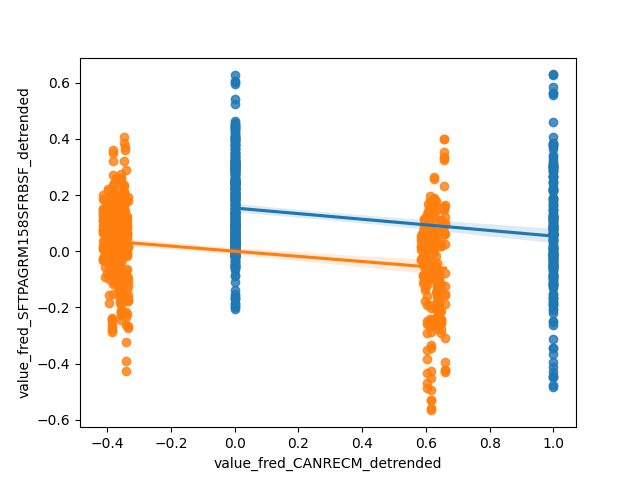
\includegraphics[scale = 0.9]{plots/plot_2026-08-20_detrended.png}
\caption{Detrended Regression Plot for 2026-08-20}
\end{figure}
\newpage
